\section{Konzept} 

\begin{frame}[c]
    \frametitle{Konzept: Framework-Klassen}
      
    \begin{figure}[t]
      %\centering
      \vspace{-0.8cm}
      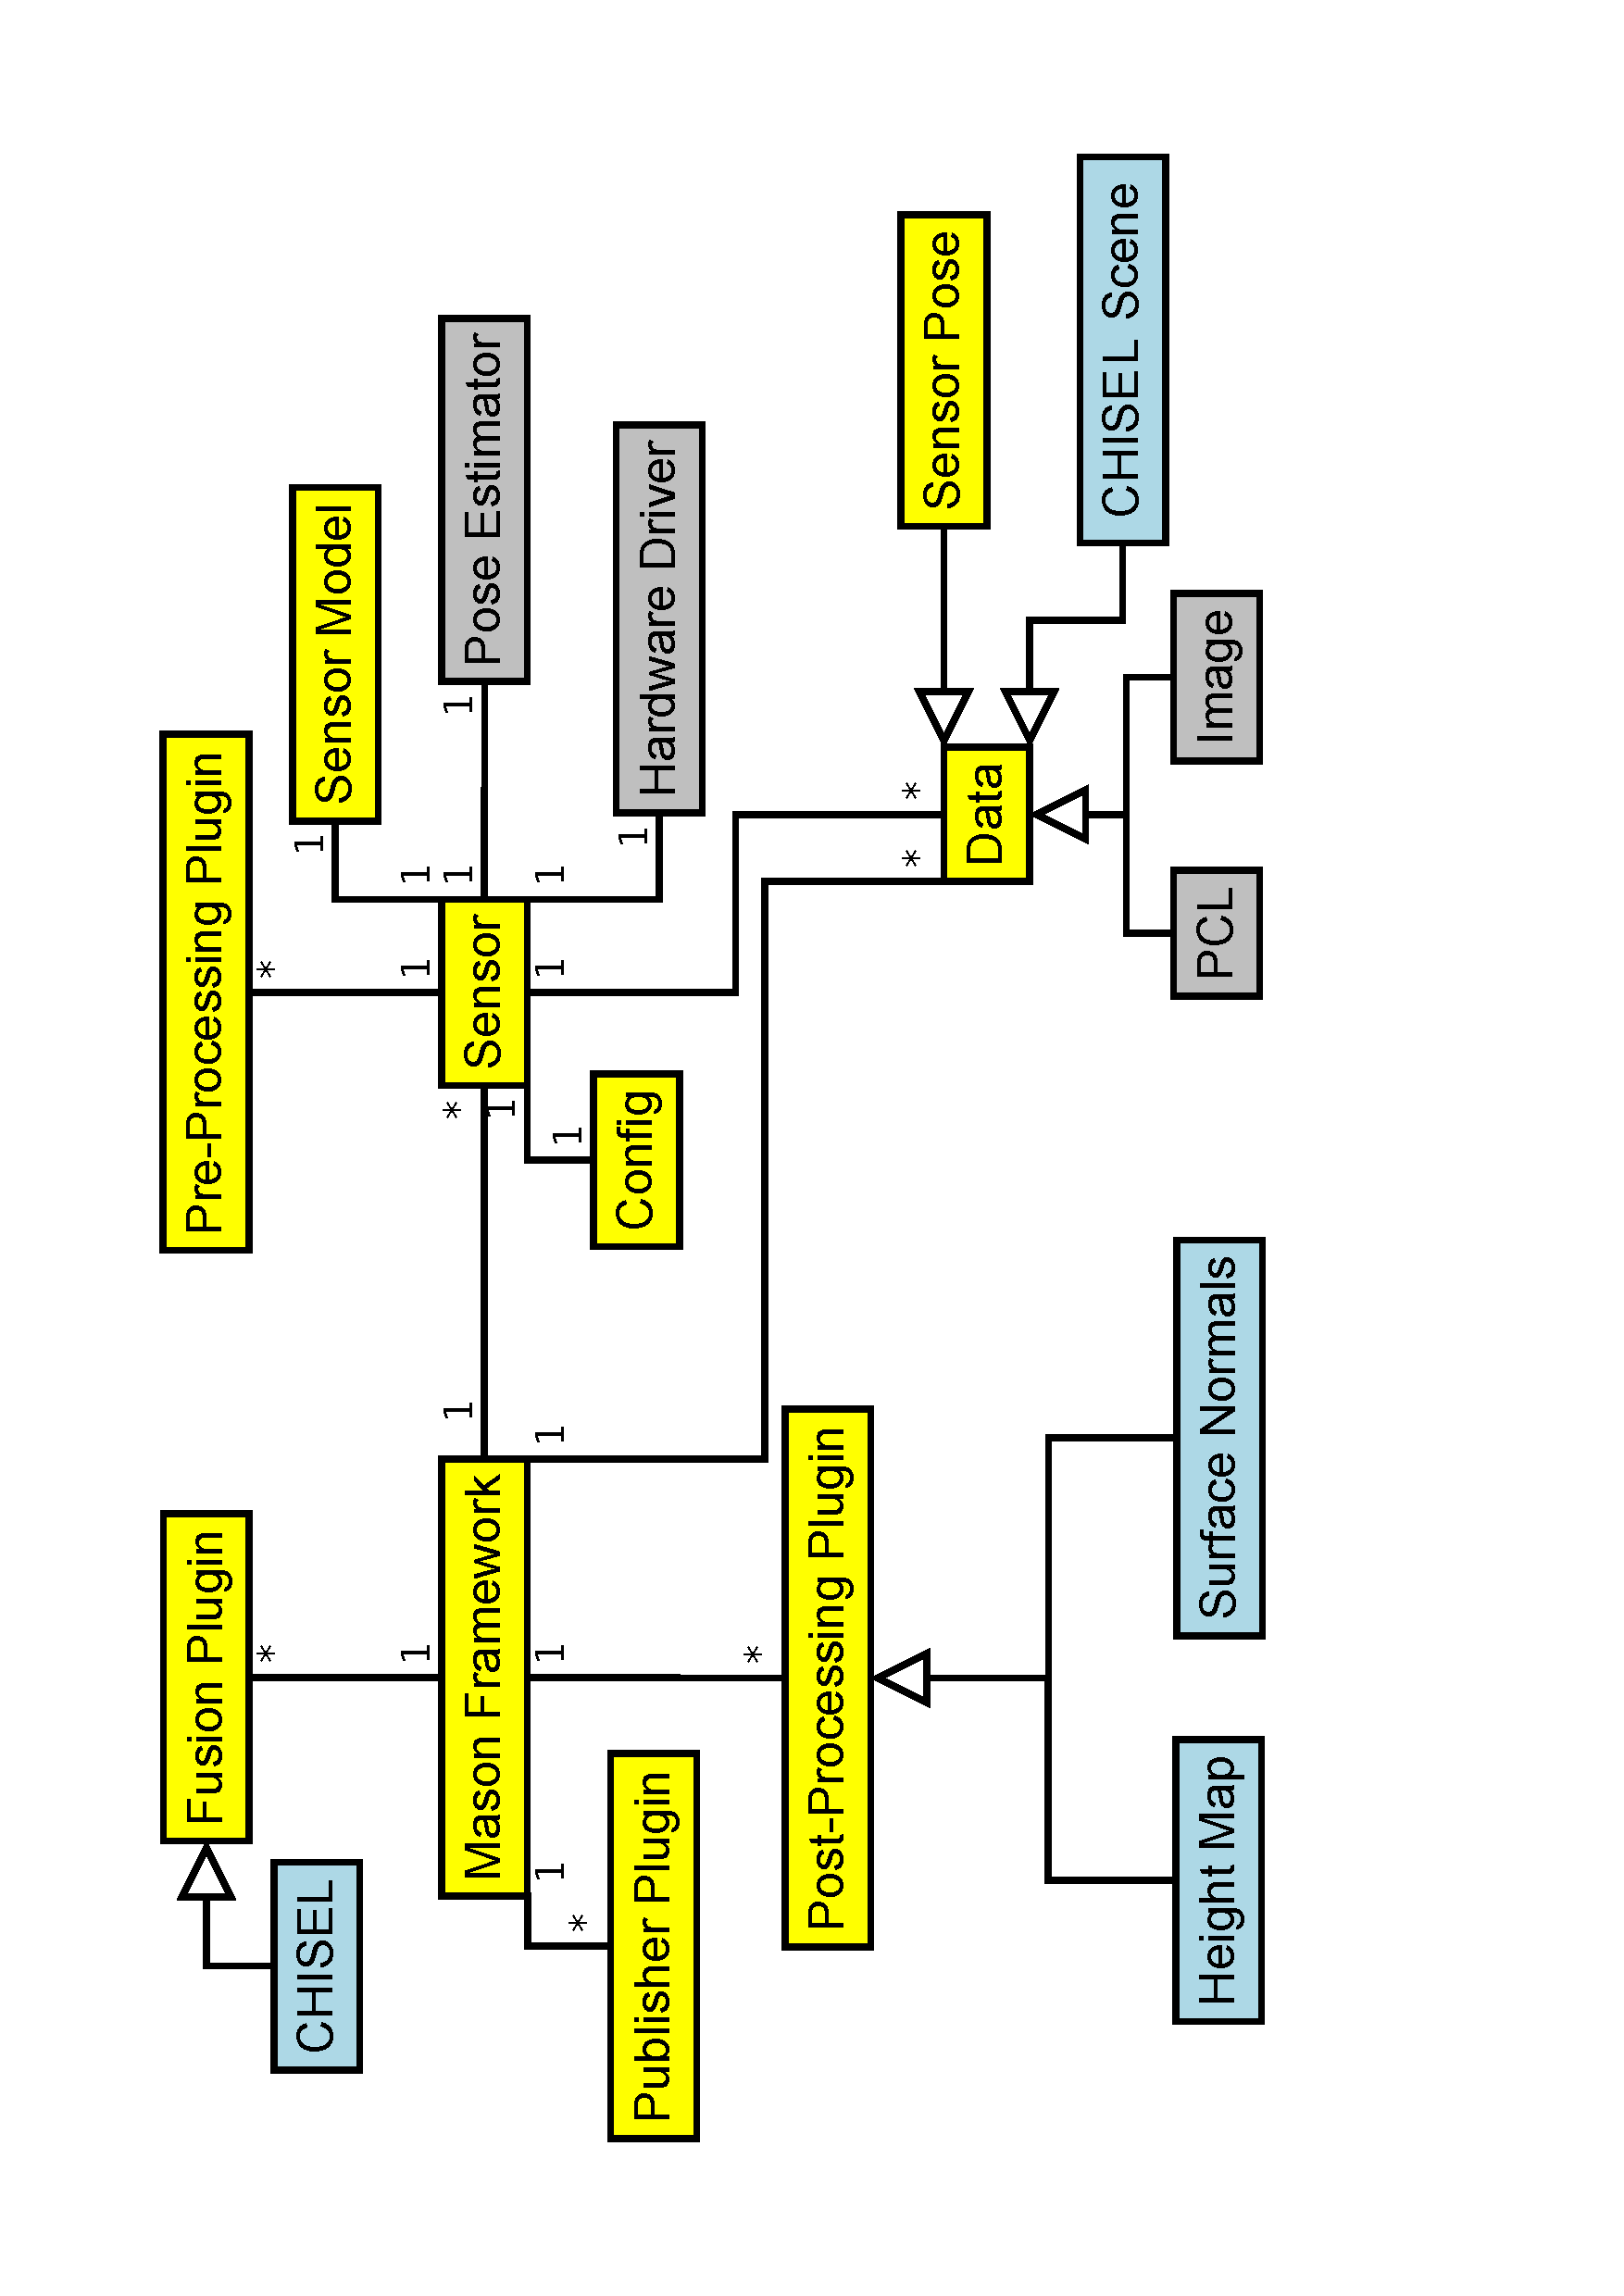
\includegraphics[angle=270,origin=c, width= \textwidth]{diagrams/framework_concept.pdf}
      \label{fig:preprocessing_phase}
    \end{figure}
 
    \end{frame}


\begin{frame}[c]
    \frametitle{Konzept: Pipeline}
      
    \begin{figure}[t]
      %\centering
      \vspace{-0.8cm}
      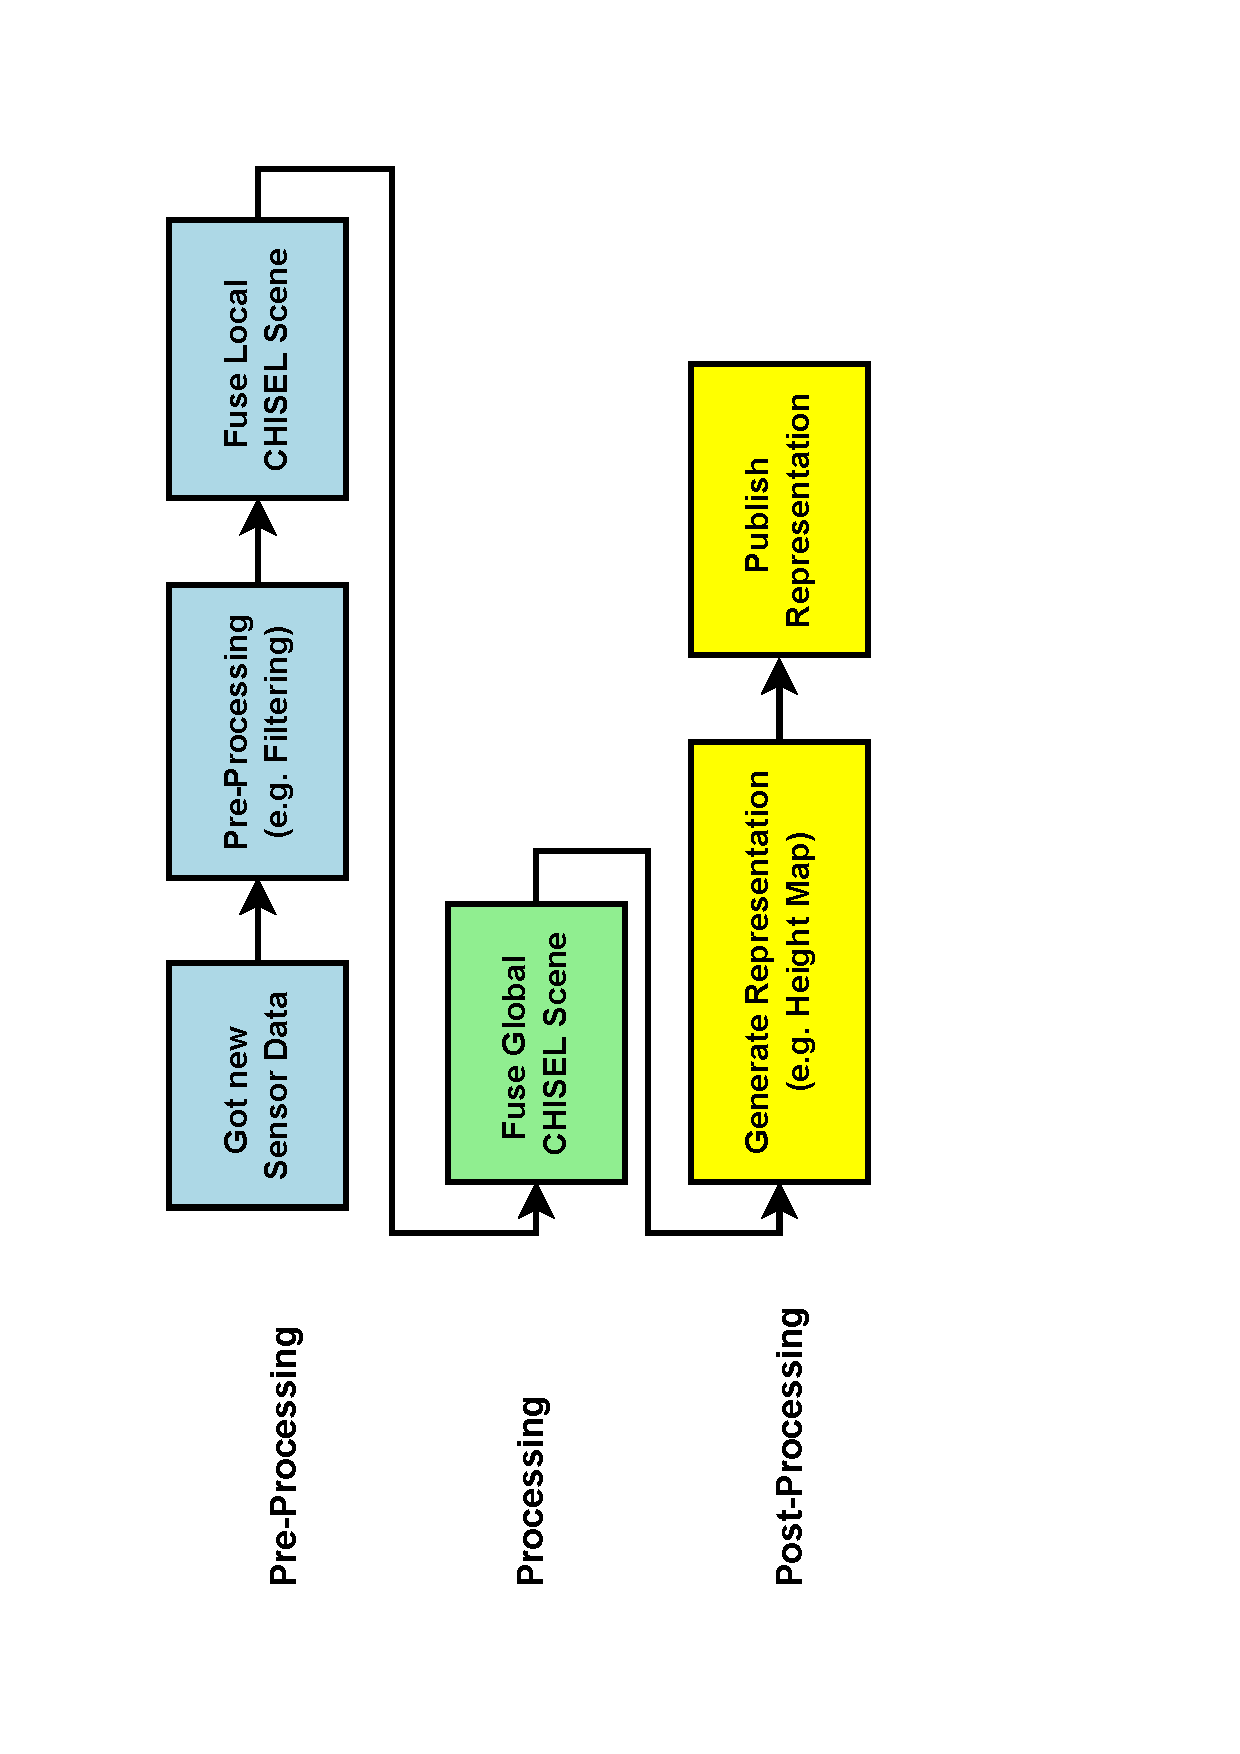
\includegraphics[angle=270,origin=c, width= \textwidth]{diagrams/pipeline.pdf}
      \label{fig:preprocessing_phase}
    \end{figure}
 
\end{frame}

\section{Aktueller Stand und Aussicht}

    \begin{frame}[t]
    \frametitle{Aktueller Stand und Aussicht}
      
      \begin{columns}[t]
      \column{5cm}
     \begin{itemize}
     \item Fusion von verschiedenen Sensoren möglich \\ $\rightarrow$ CHISEL Fusion-Plugin
      \begin{itemize}
	\item  Beliebige Voxelblock-Größen und Auflösungen
	\item  Auch mit Farbinformationen
	\item  Oberflächennormalen-Schätzung 
      \end{itemize}
     \item Tiefenbilder und Pointclouds integrierbar

      \end{itemize}
     
     \column{7cm}
      
       \begin{figure}[h]
 	\centering
 	    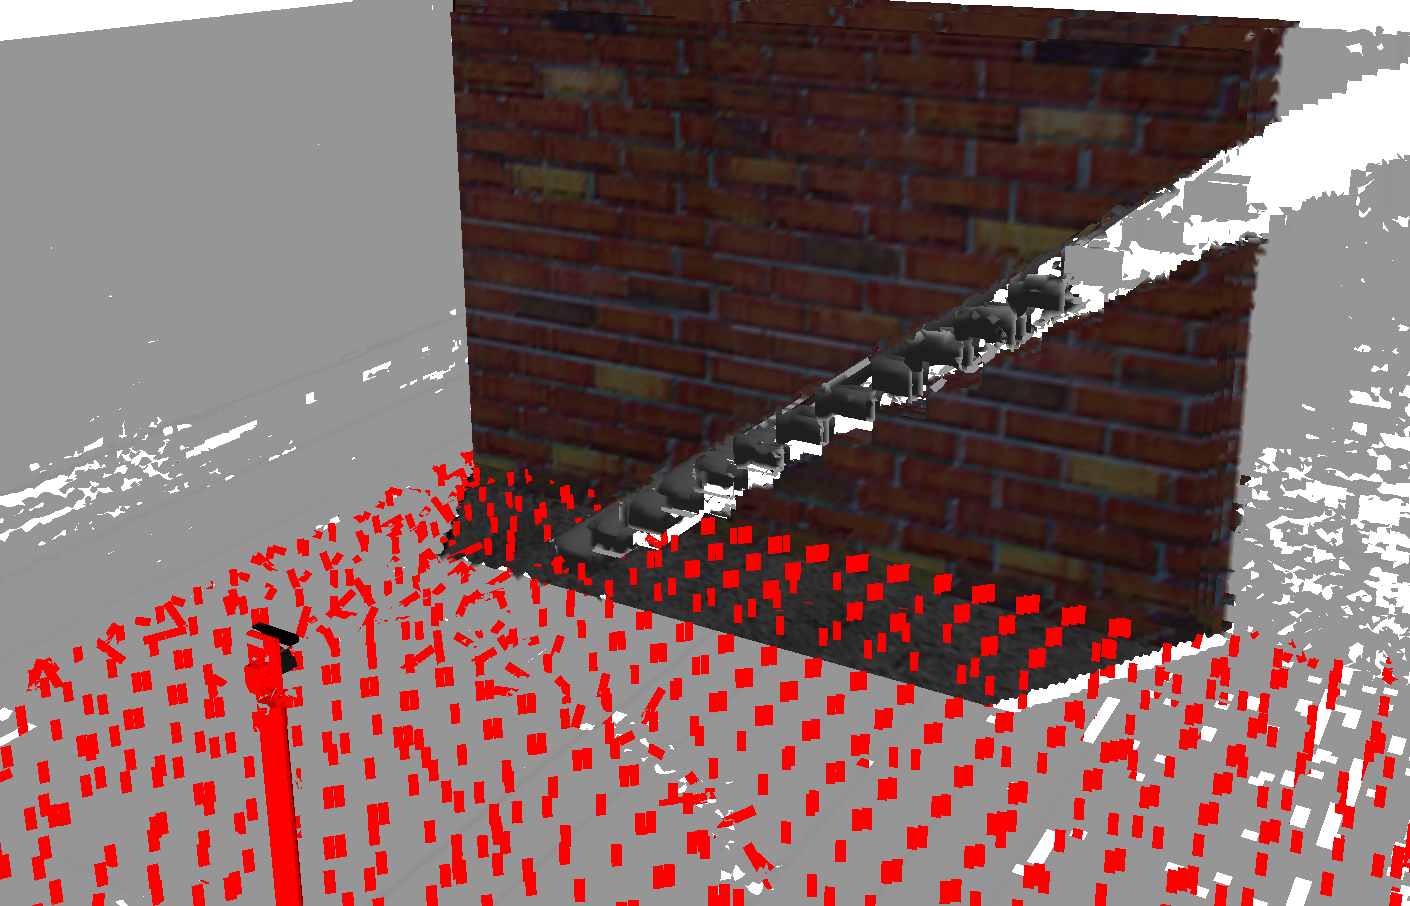
\includegraphics[width=0.9\textwidth]{images/mason_trim}
 	\caption{Fusion von RGB-D- und Laserscanner-Daten} 
       \end{figure}
  
    \end{columns}
     
    \end{frame}

\begin{frame}[c]
    \frametitle{Zusammenfassung und Aussicht}
      

    \begin{block}{Zusammenfassung}
      \begin{itemize}
       \item CHISEL als performante Basis für Multisensor-Fusions-Framework
       \item Spatially-hashed TSDF 
       \item Erstellung von verschiedenen Repräsentationen aus Weltmodell
      \end{itemize}

    \end{block}


      \begin{block}{Aussicht}
	\begin{itemize}
	  \item Implementierung vom Framework
	  \begin{itemize}
	   \item Übertragen vom aktuellen Stand in Plugins
	   \item Interface vom Framework zu CHISEL
	   %\item Fehler ausbessern

	  \end{itemize}

	  \item Evaluation
	  \begin{itemize}
	   \item Leistung
	   \item Zusammenspiel verschiedener Sensorkonfigurationen (Gazebo und Roboter)
	   \item Zuverlässigkeit
	  \end{itemize}

	\end{itemize} 
      
      \end{block}
    
    

\end{frame}